\documentclass{article}
\usepackage[utf8]{inputenc}
\usepackage[margin=1.0in]{geometry}
\usepackage{amsmath}
\usepackage{graphicx}
\usepackage{wrapfig}

\title{Transformations}
\author{Alexey Didenkov, George Tang}
\date{October 2, 2019}

\begin{document}

\maketitle

\section{Introduction}
In this lecture we'll explore both 2D and 3D transformations, and see how they can be applied to computer vision, graphics, and machine learning. 

In mathematics we use the notation $\mathbf R^n$ to represent real coordinate spaces of $n$ dimensions. For example, $\mathbf R^1$ is a number line, and $\mathbf R^3$ is a 3D space. A \texit{vector} in $\mathbf R^n$ space has $n$ components, one for each dimension. In $\mathbf R^2$ space, a vector that extends x units along the x-axis, and y units along the y-axis can be represented with row/column vector notation:
\[\mathbf{a} = \begin{bmatrix}x & y\end{bmatrix} = \begin{bmatrix}x \\y\end{bmatrix}\]
\noindent
You can think of these vectors as starting at the origin and pointing towards the points that they describe. For now, these points will be vertices of geometric shapes. This notation can also be interpreted as matrices. An $n$-dimensional vector is a 1x$n$ matrix in its row notation and a $n$x1 matrix in its column notation.

\section{2D Transformations}
The following transformations will be taking place in the 2-dimensional $\mathbf R^2$ space (plane), which means that we will be working with transformations of \mathbf{a} in the form
\[\mathbf{a}' = \begin{bmatrix}x' \\y'\end{bmatrix}\]

\subsection{Translation}
\begin{wrapfigure}{r}{0.4\textwidth}
  \begin{center}
    \vspace{-75pt}
    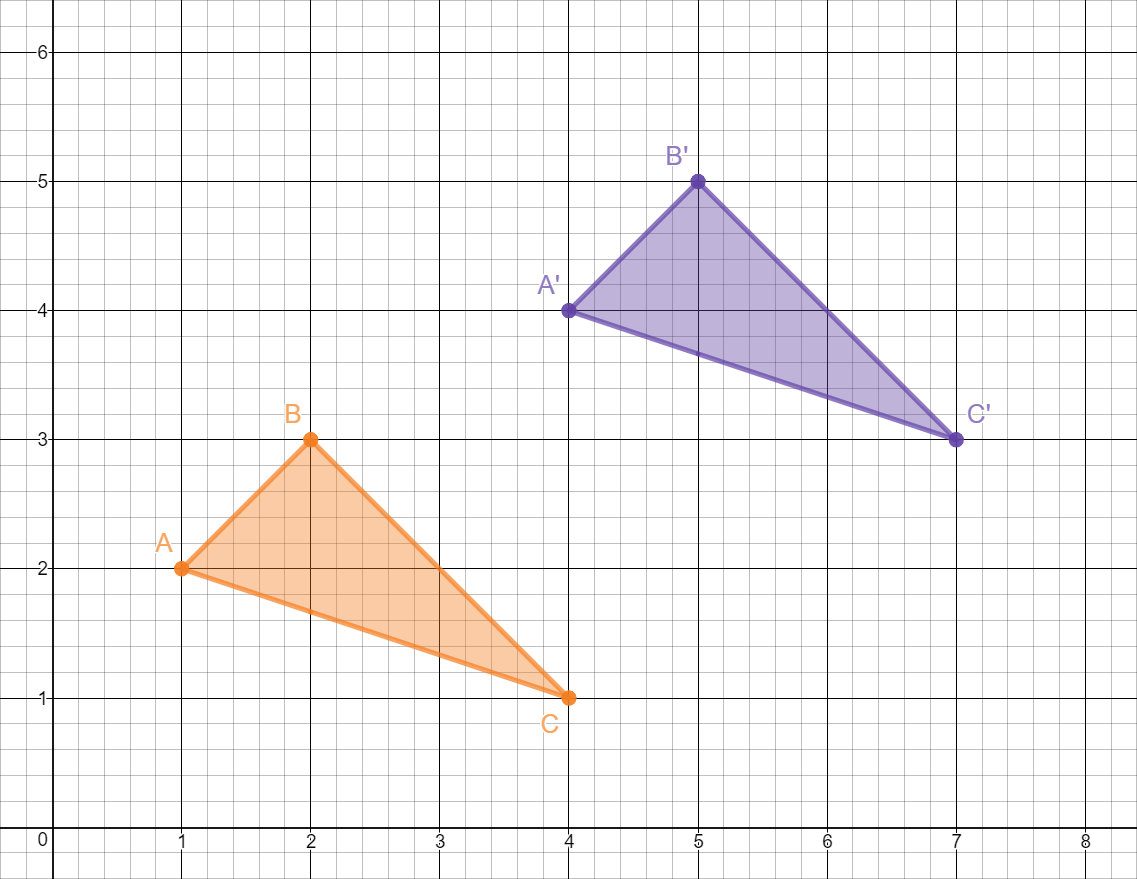
\includegraphics[width=0.30\textwidth]{2d_translation.png}
    \vspace{-17.5pt}
  \end{center}
  \caption{Translation ($\Delta x$=3, $\Delta y$=2)}
\end{wrapfigure}

Translation is when a figure is moved by $\Delta x$ in the x-direction and by $\Delta y$ in the y-direction:
\[x' = x + \Delta x\]
\[y' = y + \Delta y\]
\noindent
These equations can be expressed as matrices:
\[
\begin{bmatrix}
x' \\
y'
\end{bmatrix}
=
\begin{bmatrix}
1 & 0 & \Delta x \\
0 & 1 & \Delta y
\end{bmatrix}
\begin{bmatrix}
x \\
y \\
1
\end{bmatrix}
\]
\noindent
Decomposing the matrix multiplication yields the two equations that we used to define translation. Convince yourself that this is true. Note that the vector on the right side actually has three dimensions due to the addition of a 1 at its bottom. This this is because in translation, the constants $\Delta x$ and $\Delta y$ are added to all coordinates, regardless of what x and y are. Unfortunately, this makes our transformed vector dimensionally different. To fix this, we similarly extend the left side vector by including the equation $1=1\times1$:
\[
\begin{bmatrix}
x' \\
y' \\
1
\end{bmatrix}
=
\begin{bmatrix}
1 & 0 & \Delta x \\
0 & 1 & \Delta y \\
0 & 0 & 1
\end{bmatrix}
\begin{bmatrix}
x \\
y \\
1
\end{bmatrix}
\]
\noindent
Translation completely preserves the figure and its orientation.

\subsection{Scaling}
\begin{wrapfigure}{r}{0.4\textwidth}
  \begin{center}
    \vspace{-75pt}
    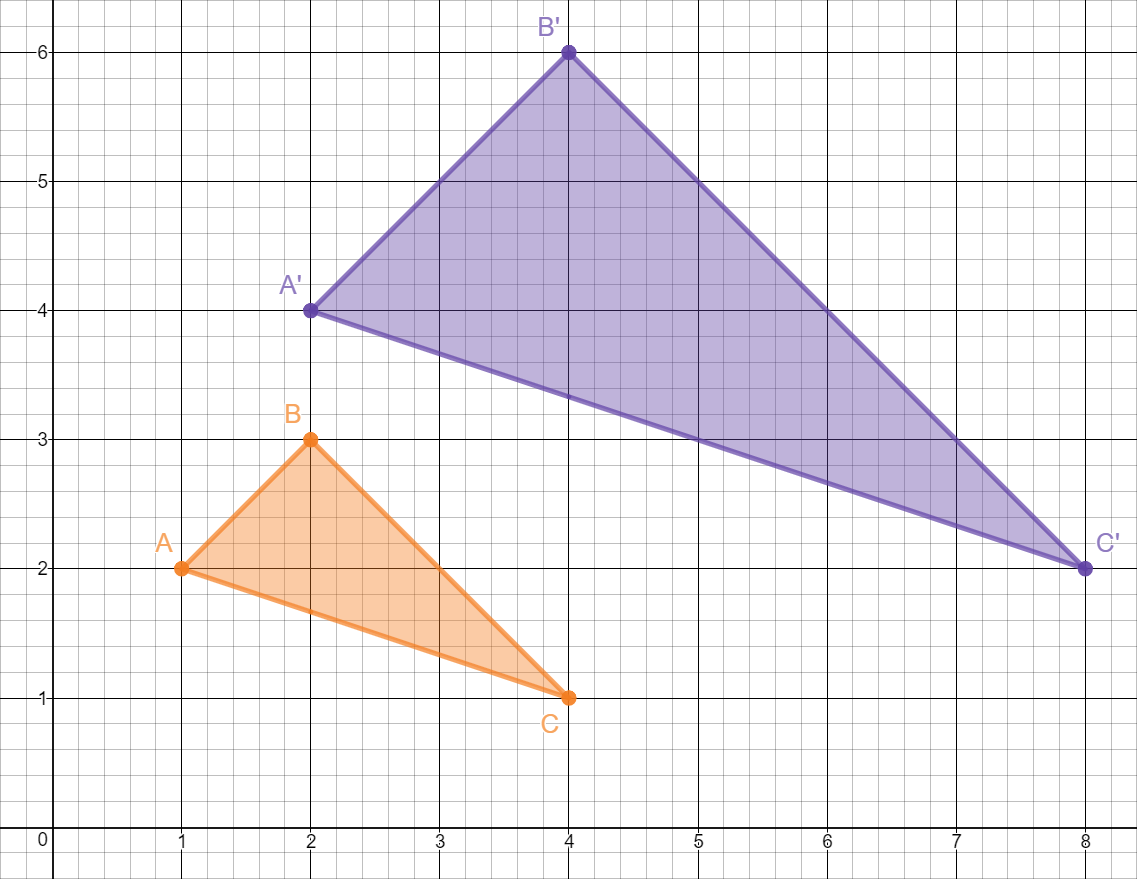
\includegraphics[width=0.3\textwidth]{2d_scaling.png}
    \vspace{-17.5pt}
  \end{center}
  \caption{Scaling ($Sx$=2, $Sy$=2)}
\end{wrapfigure}

Scaling involves multiplying every x-coordinate by $Sx$ and every y-coordinate by $Sy$, which "stretches" or "shrinks" the figure along either axis.
\[x' = Sx\times x\]
\[y' = Sy\times y\]
\noident
Let's also rewrite this transformation with matrices. Unlike translation, the equation for scaling does not contain any constants, and so all our vectors can be left as 2-dimensional. However, we'll add that third dimension to keep consistency, as we may want to stack transformations:
\[
\begin{bmatrix}
x' \\
y' \\
1
\end{bmatrix}
=
\begin{bmatrix}
Sx & 0 & 0 \\
0 & Sy & 0 \\
0 & 0 & 1
\end{bmatrix}
\begin{bmatrix}
x \\
y \\
1
\end{bmatrix}
\]
\noindent
Scaling creates a similar figure with identical orientation.

\subsection{Rotation}
\begin{wrapfigure}{r}{0.4\textwidth}
  \begin{center}
    \vspace{-70pt}
    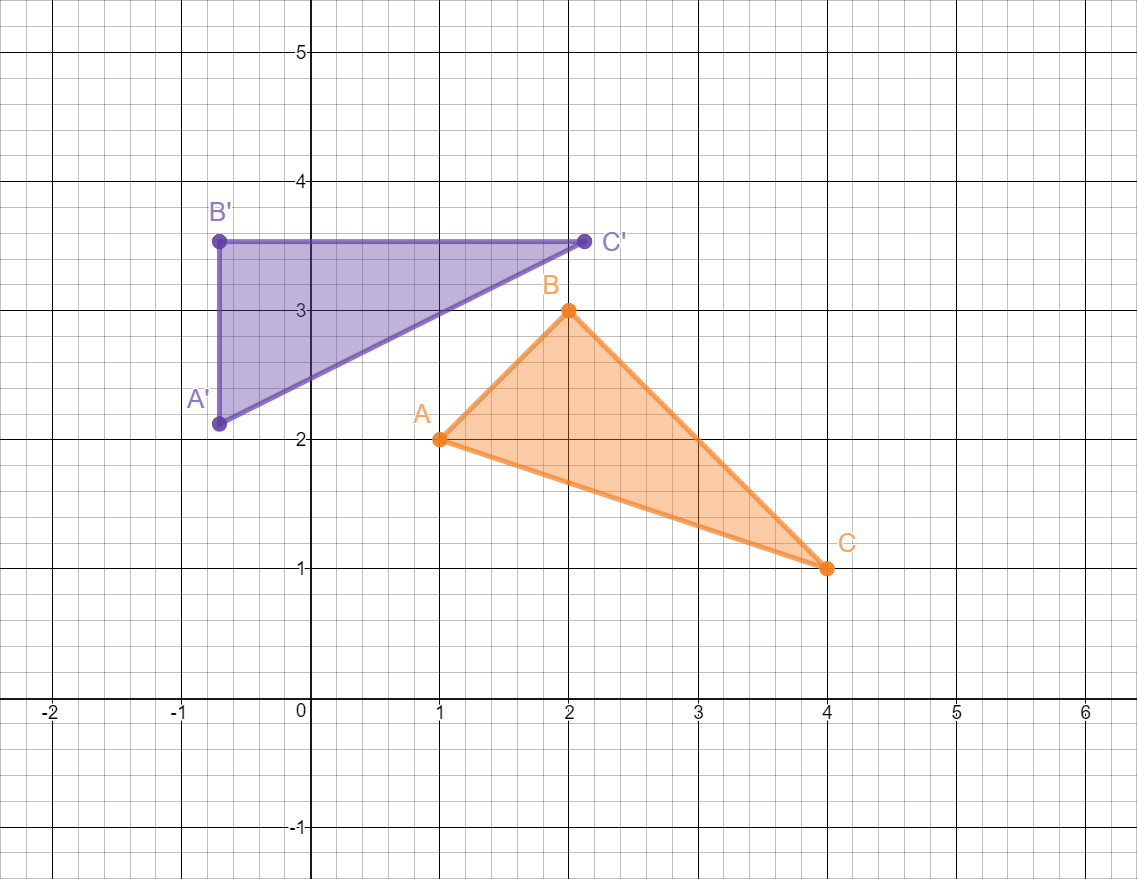
\includegraphics[width=0.30\textwidth]{2d_rotation.png}
    \vspace{-12.5pt}
  \end{center}
  \caption{Rotation ($\theta$=$\pi/2$)}
\end{wrapfigure}

Consider the point ($x$, $y$) located on the xy-plane. As we've done previously, let's think of it as a vector, but this time let's also denote its magnitude as $R$ and its angle from the positive x-axis as $\phi$. It holds true that:
\[x = R \cos \phi\]
\[y = R \sin \phi\]
\noindent
Now we're going to rotate it around the origin by $\theta$ radians counter-clockwise. Its new position, ($x'$, $y'$) will be a vector with the same magnitude $R$, but with a new angle \\
$\phi + \theta$. Substituting, expanding, and then substituting in the first two equations:, we get:

\[x' = R \cos ( \phi + \theta ) = R \cos \phi \cos \theta - R \sin \phi \sin \theta\]
\[y' = R \sin ( \phi + \theta ) = R \sin \phi \cos \theta + R \cos \phi \sin \theta\]
\[x' = x \cos \theta - y \sin \theta\]
\[y' = y \cos \theta + x \sin \theta\]
\noindent
Once again, we can represent this in matrix form, keeping in mind the third dimension for consistency:
\[
\begin{bmatrix}
x' \\
y' \\
1
\end{bmatrix}
=
\begin{bmatrix}
\cos \theta & -\sin \theta & 0 \\
\sin \theta & \cos \theta & 0 \\
0 & 0 & 1
\end{bmatrix}
\begin{bmatrix}
x \\
y \\
1
\end{bmatrix}
\]
\noindent
Rotation preserves the figure but not its orientation

\begin{figure}[!htb]
    \begin{center}
        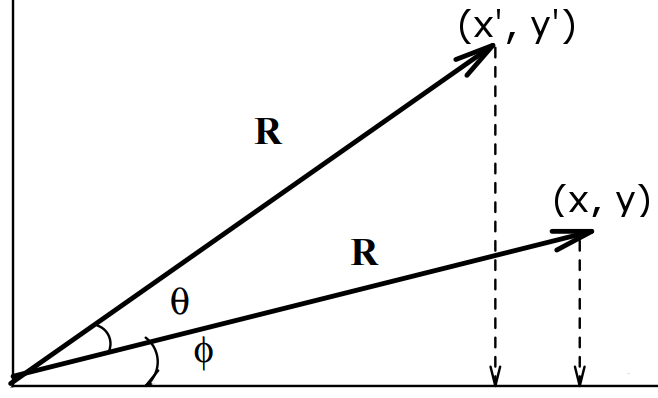
\includegraphics[width=0.30\textwidth]{rotation_triangle_flat.png}
        \vspace{-20pt}
    \end{center}
    \caption{Rotation Triangle}
\end{figure}

\subsection{Transformation Matrices and Cascading}

What if we wanted to perform several transformations at once? This would be identical to performing one transformation and using its result in the second. We can keep on \textit{cascading} transformations like this indefinitely. Recall that matrix multiplication is not commutative, so keep in mind that the order of transformations matters, and when reading an equation the order goes from right to left. But it is associative. That means that we can multiply $T_2$ by $T_1$ then the input vector and get the same result if we multiplied the input vector by $T_1$ and then $T_2$. The total transformation matrix is unique. With that in mind, let's create the general equation for transformations in 2D where $T$ is called the transformation matrix:
\[
\begin{bmatrix}
x' \\
y' \\
1
\end{bmatrix}
=
T
\begin{bmatrix}
x \\
y \\
1
\end{bmatrix}
\]
\noident
For example, the matrix for translating a figure and \textbf{then} scaling it would be:

\[
\begin{bmatrix}
Sx & 0 & 0 \\
0 & Sy & 0 \\
0 & 0 & 1
\end{bmatrix}
\begin{bmatrix}
1 & 0 & \Delta x \\
0 & 1 & \Delta y \\
0 & 0 & 1
\end{bmatrix}
=
\begin{bmatrix}
Sx & 0 & Sx\Delta x \\
0 & Sy & Sy\Delta y \\
0 & 0 & 1
\end{bmatrix}
\]
\noindent
Also, recall that matrices have inverses, and $T^{-1}T = I$. $I$ is the identity matrix. This sequence essentially acts as an in-place transformation that does nothing to the figure. 

\subsection{Affine}
\begin{wrapfigure}{r}{0.4\textwidth}
  \begin{center}
    \vspace{-50pt}
    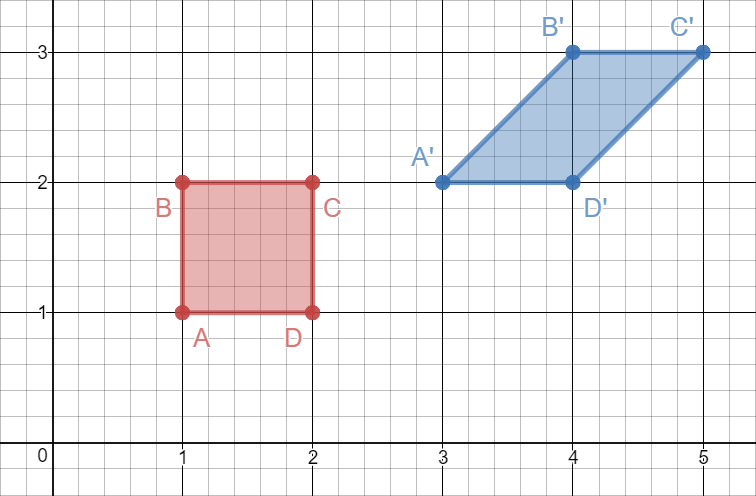
\includegraphics[width=0.30\textwidth]{2d_affine.png}
    \vspace{-20pt}
  \end{center}
  \caption{Affine Transformation}
\end{wrapfigure}

At this point you might be wondering what other wacky transformations could be created by combining translation, rotation, and scaling matrices. While there are plenty of possibilities, any transformation matrix we get as the result will create figures similar (same angles) to the original, since that is a property of every one of our underlying transformations. If we want to skew the image, we turn to affine transformations, given by the following formula\footnote{This equation can be difficult to comprehend, especially since we are no longer given pretty variables like $\Delta x$ or $\theta$. If you would like to get a better grasp on what the different $a$-variables control, we highly recommend checking out ncase.me/matrix, where you can interactively play around with the transformation matrix}:
\[
\begin{bmatrix}
x' \\
y' \\
1
\end{bmatrix}
=
\begin{bmatrix}
a_{00} & a_{01} & a_{02} \\
a_{10} & a_{11} & a_{12} \\
0 & 0 & 1 \\
\end{bmatrix}
\begin{bmatrix}
x \\
y \\
1
\end{bmatrix}
\]
\noindent
This gives us a full 6 degrees of freedom, allowing the figure to be skewed. Still, affine transformation preserves parallel lines.

\subsection{Projective}
\begin{wrapfigure}{r}{0.4\textwidth}
  \begin{center}
    \vspace{-40pt}
    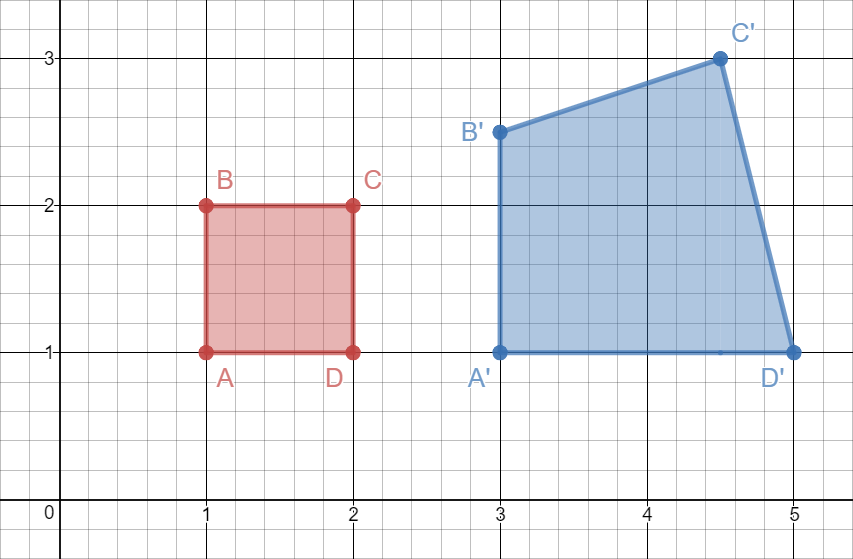
\includegraphics[width=0.30\textwidth]{2d_projective.png}
    \vspace{-20pt}
  \end{center}
  \caption{Projective Transformation}
\end{wrapfigure}

Why only stop at 6 parameters when our 3$\times$3 matrix has 9? Let's go ahead and express the new formula:
\[
\begin{bmatrix}
kx' \\
ky' \\
k
\end{bmatrix}
=
\begin{bmatrix}
h_{00} & h_{01} & h_{02} \\
h_{10} & h_{11} & h_{12} \\
h_{20} & h_{21} & h_{22} \\
\end{bmatrix}
\begin{bmatrix}
x \\
y \\
1
\end{bmatrix}
\]
\noindent
Now, hold on a minute, what is this $k$ that the output vector is multiplied by? Turns out, that the identity statement that we used to "add the 1" to the vectors no longer holds true. Here, the bottom-most term becomes $k = h_{20}x + h_{21}y + h_{22}$.
This makes our vectors \textbf{homogeneous} (denoted as $\mathbf{\tilde a}$), meaning that their last parameter is not 1. To convert homogeneous vectors back, you just have to divide the entire vector by its last parameter. In our case:

\[
\begin{bmatrix}
kx' \\
ky' \\
k
\end{bmatrix}
/ k = 
\begin{bmatrix}
x' \\
y' \\
1
\end{bmatrix}
\]
\[
k
\begin{bmatrix}
x' \\
y' \\
1
\end{bmatrix}
=
\begin{bmatrix}
h_{00} & h_{01} & h_{02} \\
h_{10} & h_{11} & h_{12} \\
h_{20} & h_{21} & h_{22} \\
\end{bmatrix}
\begin{bmatrix}
x \\
y \\
1
\end{bmatrix}
\]
\noindent
Note how this makes our 3$\times$3 matrix indifferent to scale - two matrices that differ only by scale will produce the same output vector (due to division by $k$) and are thus equivalent. This allows us to say that the transformation matrix is also homogeneous.

Projective transform only preserves straight lines.

\subsection{Applications}
Perhaps the largest application of 2D transformations is \textbf{transforming images}. On the most fundamental level, images are flat 2D arrays of pixels, discrete minuscule areas represented by a coordinate and a color. We can interpret that coordinate much like we did vertices previously, and perform all of the above-mentioned operations without touching the pixels' color. The procedure looks something like this:\\

For every pixel $a$ in $f(a)$:
\begin{enumerate}
\item Compute its destination location $a' = T\times a$
\item Copy the pixel $f(a)$ to $g(a')$
\end{enumerate}

However, there are some glaring problems. The domains of the original and its image might not match, leaving some background unfilled. Also, the new locations might not be discrete - we will most likely end up with decimal values for coordinates. One solution is to "spread" the pixel over the nearest integer coordinates, a technique called \textit{splatting}. However, doing so will result in a blur and loss of information. A better solution is to modify our procedure to "work backwards":\\

For every pixel $a'$ in $g(a')$:
\begin{enumerate}
\item Compute the source location $a = T^{-1}\times a'$
\item Resample $f(a)$ at location $a$ and copy to $g(a')$
\end{enumerate}

There are plenty more details to this procedure, and we recommend looking into them if you are interested. If you are not then don't fret - most libraries will have already implemented this for you. For example, OpenCV provides a method that transforms an images based on a given transformation matrix. The result looks something like this:

\begin{figure}[!htb]
    \begin{center}
        \vspace{-8pt}
        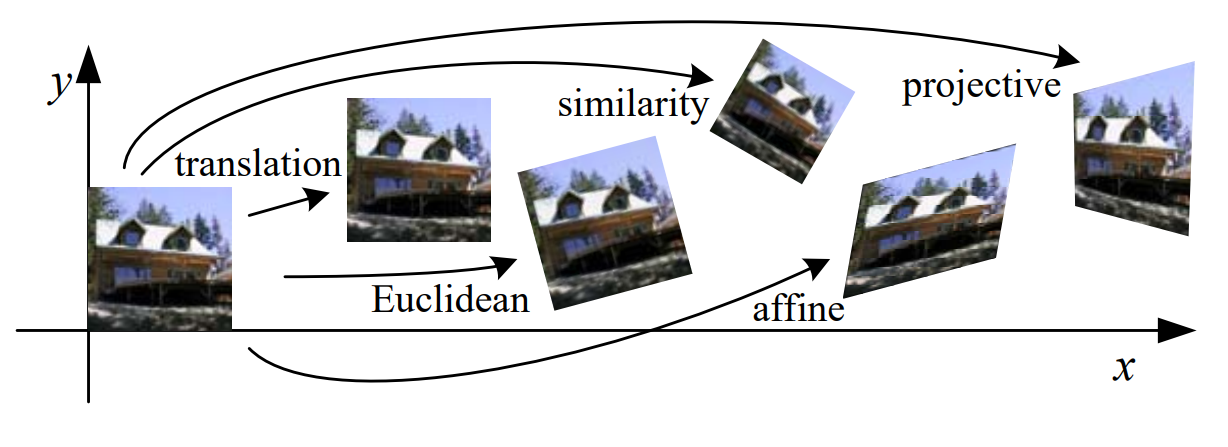
\includegraphics[width=0.5\textwidth]{2d_image_transformations.png}
        \vspace{-30pt}
    \end{center}
    \caption{2D Image Transformations}
\end{figure}

Now, what can we do with this newfound power? \textit{Supervised learning} is a popular branch of machine learning, but it requires a lot of labeled data, which is not often easy or cheap to come by. As a result, a popular technique developed called \textbf{data augmentation}, which is especially effective when working with images. The premise is simple: you can copy the images that you already have but modify them slightly. This is where image transformations come in: you can use rotations, translations, scaling, or even mirror the images. This way, you get images with the same label and depicting the same object, only they look completely different to your model. Doing so often allows you to better train networks on small amounts of data while avoiding overfitting.

\begin{figure}[!htb]
    \begin{center}
        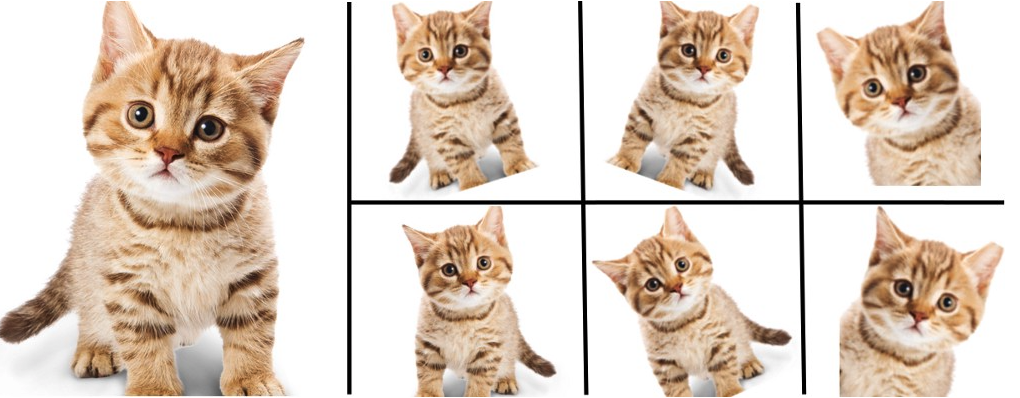
\includegraphics[width=0.45\textwidth]{kitty_augmentation.png}
        \vspace{-20pt}
    \end{center}
    \caption{Data Augmentation}
\end{figure}

As another example, let's suppose that you are making an AI that can look at license plates of cars and be able to read them. You've worked hard to produce a model that works really well when reading license plates head-on, but struggles in the real world, as most pictures you find of real cars have their plates at an angle or warped due to perspective. The solution to this is to perform \textbf{inverse projective transform}. If you can find the corners of the license plate, the rest is as simple as performing projective transform to undo the effect of real-life perspective, thus getting a flat view of the license plate.

\begin{figure}[!htb]
    \begin{center}
        
\includegraphics[width=0.55\textwidth]{ferrari2.jpg}
        \vspace{-20pt}
    \end{center}
    \caption{Inverse Projective Transform}
\end{figure}

\section{3D Transformations}
Transformation equations in 3D are mostly similar to their 2D counterparts. The main difference happens to be the addition of a z-value to the vectors, which makes them 4$\times$1:

\[
a = 
\begin{bmatrix}
x \\
y \\
z \\
1
\end{bmatrix}
,\quad
a' = 
\begin{bmatrix}
x' \\
y' \\
z' \\
1
\end{bmatrix}
\]
\noindent
We still keep that 1 at the bottom of both vectors. This means that our transformation matrices now become 4$\times$4. The new equations for translation and scaling, respectively, are:
\[
\begin{bmatrix}
x' \\
y' \\
z' \\
1
\end{bmatrix}
=
\begin{bmatrix}
1 & 0 & 0 & \Delta x \\
0 & 1 & 0 & \Delta y \\
0 & 0 & 1 & \Delta z \\
0 & 0 & 0 & 1
\end{bmatrix}
\begin{bmatrix}
x \\
y \\
z \\
1
\end{bmatrix}
\]
\[
\begin{bmatrix}
x' \\
y' \\
z' \\
1
\end{bmatrix}
=
\begin{bmatrix}
Sx & 0 & 0 & 0 \\
0 & Sy & 0 & 0 \\
0 & 0 & Sz & 0 \\
0 & 0 & 0 & 1
\end{bmatrix}
\begin{bmatrix}
x \\
y \\
z \\
1
\end{bmatrix}
\]

\subsection{Rotation in 3D - Euler Angles}
Following the logical progression of the previous two extensions, let's attempt to likewise convert rotation into 3D:
\[
\begin{bmatrix}
x' \\
y' \\
z' \\
1
\end{bmatrix}
=
\begin{bmatrix}
\cos \theta & -\sin \theta & 0 & 0 \\
\sin \theta & \cos \theta & 0 & 0 \\
0 & 0 & 1 & 0 \\
0 & 0 & 0 & 1
\end{bmatrix}
\begin{bmatrix}
x \\
y \\
z \\
1
\end{bmatrix}
\]

Unlike the previous statements, which saw the addition of terms like $\Delta z$ and $Sz$, the new rotation equation is nearly identical to its 2D counterpart, aside from the addition of $z' = z$. This means that the equation will perform exactly like it did in 2D, additionally making sure to preserve values in the z-dimension. When we did rotation back in 2D, we rotated figures CCW in the xy-plane and around the origin. Taking this into context of 3D, the new equation will rotate points CCW around the z-axis (when looking down from its positive end).

While we only had one axis to rotate around in 2D, the z-axis is only one of three possible discrete axes to choose from in 3D. Thus, let's call this last transformation matrix $R_z(\theta)$ and set out to find $R_x(\theta)$ and $R_y(\theta)$.

From the equation, we can see that the z-parameter is unaffected by sines and cosines during matrix multiplication. Since $z$ is third from the top in $\mathbf a$ and the third column of $R_z(\theta)$ is mostly empty, $z$ does not get multiplied with any trig functions. Similarly, since $z'$ is third from the top in $\mathbf a'$ and the third row of $R_z(\theta)$ is mostly empty, the value of $z'$ does not get affected by any trig functions. The only relationship here is $z' = z$.

This unique position is what ensures that z stays the same and determines z as the rotation axis. While we could achieve the same result with both x and y by swapping the order of the variables in the vectors, let's instead elect to rearrange the transformation matrix for consistency. The goal here is to "free up" the first row and column to rotate around the x-axis, and the second row and column to rotate around the y-axis. Doing so, we get:

\[
R_x(\theta) = 
\begin{bmatrix}
1 & 0 & 0 & 0 \\
0 & \cos \theta & -\sin \theta & 0 \\
0 & \sin \theta & \cos \theta & 0 \\
0 & 0 & 0 & 1
\end{bmatrix}
,\quad
R_y(\theta) = 
\begin{bmatrix}
\cos \theta & 0 & -\sin \theta & 0 \\
0 & 1 & 0 & 0 \\
\sin \theta & 0 & \cos \theta & 0 \\
0 & 0 & 0 & 1
\end{bmatrix}
\]
\noindent
Verifying these matrices mathematically is left as an exercise for the reader. These rotation matrices can be combined together to represent any rotation in 3D space:
\[R = R _ { z } ( \alpha ) R _ { y } ( \beta ) R _ { x } ( \gamma )\]
where $\alpha$, $\beta$, $\gamma$ are yaw, pitch, and roll respectively. Recall that upon cascading, the order of transformations goes from right to left, meaning that roll is applied first, then pitch, then yaw. Using a different order will yield a different angle and a different transformation matrix - \textbf{rotation is not commutative}.

\subsection{Rotation in 3D - Axis/angle}
The previous description of rotation can be quite confusing, especially so because the order that the operations are applied in matters. It can be quite more convenient to define complex rotations not as a combination of several others along predefined axes, but rather a single rotation by $\theta$ radians along an arbitrary axis $\mathbf{\hat n}$. Let's first decompose the rotated vector $\mathbf v$ into a component parallel and a component perpendicular to $\mathbf{\hat n}$:
\[
\boldsymbol { v } _ { \| } = 
\dfrac{( \hat { \boldsymbol { n } } \cdot \boldsymbol { v } )}{\| \hat { \boldsymbol { n } } \| ^ 2} \hat { \boldsymbol { n } } = 
\hat { \boldsymbol { n } } ( \hat { \boldsymbol { n } } \cdot \boldsymbol { v } ) = 
\left( \hat { \boldsymbol { n } } \hat { \boldsymbol { n } } ^ { T } \right) \boldsymbol { v }
\]
\[
\boldsymbol { v } _ { \perp } =
\boldsymbol { v } - \boldsymbol { v } _ { \| } =
\left( \boldsymbol { I } - \hat { \boldsymbol { n } } \hat { \boldsymbol { n } } ^ { T } \right) \boldsymbol { v }
\]
\noindent
Now, let's find a 90$^\circ$ CCW rotation of $\mathbf{v_\perp}$ around $\mathbf{\hat n}$ using the cross-product. Note: even though the result is a rotation of $\mathbf{v_\perp}$, we use $\mathbf v$ in the equation to make later math easier. The additional component $\mathbf{v_\|}$ is eliminated by the cross-product and introduces no errors: 
\[
\boldsymbol { v } _ { \times } = \hat { \boldsymbol { n } } \times \boldsymbol { v } = [ \hat { \boldsymbol { n } } ]_{\times} \boldsymbol { v }
\]
\noindent
Here, $[ \hat { \boldsymbol { n } } ]_{\times}$ is the cross-product involving $\hat { \boldsymbol { n } }$ in its matrix form:
\[
[ \hat { \boldsymbol { n } } ] _ { \times } = \left[ \begin{array} { c c c } { 0 } & { - \hat { n } _ { z } } & { \hat { n } _ { y } } \\ { \hat { n } _ { z } } & { 0 } & { - \hat { n } _ { x } } \\ { - \hat { n } _ { y } } & { \hat { n } _ { x } } & { 0 } \end{array} \right]
\]
\noindent
Now, rotate the result by 90$^\circ$ to get a total rotation of 180$^\circ$:
\[
\boldsymbol { v } _ { \times \times } = \hat { \boldsymbol { n } } \times \boldsymbol { v } _ { \times } = [ \hat { \boldsymbol { n } } ] _ { \times } ^ { 2 } \boldsymbol { v } = 
- \boldsymbol { v } _ { \perp }
\]
\noindent
Knowing this, let's rewrite our first equation:
\[
\boldsymbol { v } _ { \| } = 
\boldsymbol { v } - \boldsymbol { v } _ { \perp } = \boldsymbol { v } + \boldsymbol { v } _ { \times \times } = 
\left( \boldsymbol { I } + [ \hat { \boldsymbol { n } } ] _ { \times } ^ { 2 } \right) \boldsymbol { v }
\]
\noindent
Finally, let's find the rotated version of $\mathbf{v_\perp}$, represented by $\mathbf{u_\perp}$:
\[
\boldsymbol { u } _ { \perp } = 
\cos \theta \boldsymbol { v } _ { \perp } + \sin \theta \boldsymbol { v } _ { \times } = 
\left( \sin \theta [ \hat { \boldsymbol { n } } ] _ { \times } - \cos \theta [ \hat { \boldsymbol { n } } ] _ { \times } ^ { 2 } \right) \boldsymbol { v }
\]
\noindent
Now, let's find $\mathbf u$. Since $\mathbf{v_\|}$ is parallel to $\mathbf{\hat n}$, it will not be affected in the rotation and can be substituted in place of $\mathbf{u_\|}$:
\[
\boldsymbol { u } = 
\boldsymbol { u } _ { \perp } + \boldsymbol { v } _ { \| } = 
\left( \sin \theta [ \hat { \boldsymbol { n } } ] _ { \times } - \cos \theta [ \hat { \boldsymbol { n } } ] _ { \times } ^ { 2 } \right) \boldsymbol { v } + \left( \boldsymbol { I } + [ \hat { \boldsymbol { n } } ] _ { \times } ^ { 2 } \right) \boldsymbol { v } = 
\left( \boldsymbol { I } + \sin \theta [ \hat { \boldsymbol { n } } ] _ { \times } + ( 1 - \cos \theta ) [ \hat { \boldsymbol { n } } ] _ { \times } ^ { 2 } \right) \boldsymbol { v }
\]
\noindent
You might recognize this equation from our definition of transformations ($u = Rv$, a.k.a. $a' = Ta$). So, let's finally extract this middle matrix that defines the rotation:
\[
\boldsymbol { R } ( \hat { \boldsymbol { n } } , \boldsymbol { \theta } ) = \boldsymbol { I } + \sin \theta [ \hat { \boldsymbol { n } } ] _ { \mathrm { x } } + ( 1 - \cos \theta ) [ \hat { \boldsymbol { n } } ] _ { \mathrm { x } } ^ { 2 }
\]
\noident
This is known as \textit{Rodriguez’s formula}. In matrix form, it looks like so:
\[
\begin{bmatrix}
x' \\
y' \\
z' \\
1
\end{bmatrix}
=
\begin{bmatrix}
\cos \theta + \hat { n } _ { x } ^ { 2 } ( 1 - \cos \theta ) & \hat { n } _ { x } \hat { n } _ { y } ( 1 - \cos \theta ) - \hat { n } _ { z } \sin \theta & \hat { n } _ { y } \sin \theta + \hat { n } _ { x } \hat { n } _ { z } ( 1 - \cos \theta ) & 0 \\
\hat { n } _ { z } \sin \theta + \hat { n } _ { x } \hat { n } _ { y } ( 1 - \cos \theta ) & \cos \theta + \hat { n } _ { y } ^ { 2 } ( 1 - \cos \theta ) & - \hat { n } _ { x } \sin \theta + \hat { n } _ { y } \hat { n } _ { z } ( 1 - \cos \theta ) & 0 \\
- \hat { n } _ { y } \sin \theta + \hat { n } _ { x } \hat { n } _ { z } ( 1 - \cos \theta ) & \hat { n } _ { x } \sin \theta + \hat { n } _ { y } \hat { n } _ { z } ( 1 - \cos \theta ) & \cos \theta + \hat { n } _ { z } ^ { 2 } ( 1 - \cos \theta ) & 0 \\
0 & 0 & 0 & 1
\end{bmatrix}
\begin{bmatrix}
x \\
y \\
z \\
1
\end{bmatrix}
\]
\noident
For small $\theta$, $sin{\theta} \approx \theta$ and $cos{\theta} \approx 1$. Defining $\boldsymbol \omega = \theta \boldsymbol{ \hat n }$, the transformation matrix simplifies to:
\[
\boldsymbol { R } ( \boldsymbol { \omega } ) \approx \boldsymbol { I } + \sin \theta [ \hat { \boldsymbol { n } } ] _ { \boldsymbol { x } } \approx \boldsymbol { I } + [ \theta \hat { \boldsymbol { n } } ] _ { \mathbf { x } } = \left[ \begin{array} { c c c c } { 1 } & { - \omega _ { z } } & { \omega _ { y } } & { 0 } \\ { \omega _ { z } } & { 1 } & { - \omega _ { x } } & { 0 } \\ { - \omega _ { y } } & { \omega _ { x } } & { 1 } & { 0 } \\ { 0 } & { 0 } & { 0 } & { 1 } \end{array} \right]
\]
\noident
While regular rotation is not commutative, these minuscule rotations are. This unlocks another way to derive \textit{Rodriguez’s formula}: one rotation by $\theta$ is then equivalent to k rotations by $\theta / k$. We can take the limit of this expression as $k\to\infty$ and expand its Taylor series to get the familiar equation. This technique is called \textit{exponential twist}.

\subsection{Applications}
Similarly to how we could use 2D transformations on figures lying in a plane, we can use their 3D versions to move around three-dimensional geometric shapes. Just like their 2D counterparts, these new shapes are represented by a collection of vertices, and transforming the shape is equivalent to transforming each vertex.

As it turns out, almost all 3D models in the real world are represented this way. Even the more complex solids are represented by the surface that encloses them, which in turn is stored as a collection of vertices. Such models are often found in \textbf{gaming}, \textbf{movies}, and \textbf{computer-aided design}. Thus, 3D transformations are immensely useful when moving around these models in the simulated world, whether it involves moving a character on screen, or moving a finished part to its correct place in an OnShape assembly.

\section{3D to 2D Transformations}
Up until now, we've looked at both 2D and 3D transformations, but we've only done so separately. In reality, our 3D world is often represented in 2D - through pictures, photos, monitors, etc. This is because our visual system is 2D in itself, so it only makes sense if we could perform the same operation our eyes do, but digitally.

\subsection{Pinhole Camera}
\begin{wrapfigure}{r}{0.5\textwidth}
  \begin{center}
    \vspace{-55pt}
    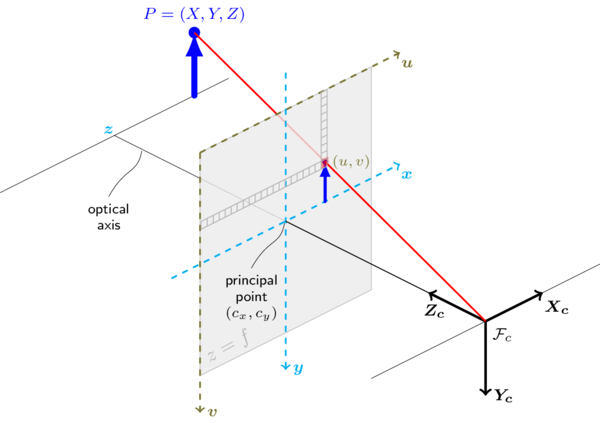
\includegraphics[width=0.4\textwidth]{pinhole_camera_model.png}
    \vspace{-15pt}
  \end{center}
  \caption{Pinhole Camera Model}
\end{wrapfigure}

Since we're basing this transformation on the way our eyes perceive reality, we need to constraint the transformation the same ways that our eyes do. Recall from the previous lecture we can model this as the pinhole camera.

\subsection{Homogeneous Coordinates}
Recall how, when we did 2D projective transform, we ended up with a homogeneous vector - the extra dimension of it was $k$ rather than 1. We got rid of it by dividing the vector by $k$.

Here, however, this has a few important implications. First of all, 2D homogeneous coordinates can represent points in 3D space. If we define our focal point to be the origin, and our image plane to be the plane $z=1$ (looking in the +z direction), we can imagine these points as representing the $x$ and $y$ values on the image plane, and the third value $k$ representing how far behind the image the points are. Second, by defining the points as such, the "divide by $k$" operation that we used before to turn a homogeneous vector to a normal one can be used to perform perspective transform where $u$ and $v$ are the coordinates on an image plane:

\[
k \left[ \begin{array} { c } { u } \\ { v } \\ { 1 } \end{array} \right] = 
\left[ \begin{array} { c } { ku } \\ { kv } \\ { k } \end{array} \right] = 
\left[ \begin{array} { c } { x } \\ { y } \\ { z } \end{array} \right]
\]

\subsection{Perspective Transform}
Now, since we're dealing with a transformation, let's make it look like one by giving it a transformation matrix:

\[
k \left[ \begin{array} { c } { u } \\ { v } \\ { 1 } \end{array} \right] = \left[ \begin{array} { c c c c } { 1 } & { 0 } & { 1 } & { 0 } \\ { 0 } & { 1 } & { 1 } & { 0 } \\ { 0 } & { 0 } & { 1 } & { 0 } \end{array} \right] \left[ \begin{array} { l } { x } \\ { y } \\ { z } \\ { 1 } \end{array} \right]
\]
\noident
But, our transformation is still lacking parameters. We can use values $f_x$ and $f_y$ to describe the size of the image plane, and $c_x$ and $c_y$ to describe where it's centered. If we do so, our equation becomes:

\[
k \left[ \begin{array} { c } { u } \\ { v } \\ { 1 } \end{array} \right] = \left[ \begin{array} { c c c c } { f _ { x } } & { 0 } & { c _ { x } } & { 0 } \\ { 0 } & { f _ { y } } & { c _ { y } } & { 0 } \\ { 0 } & { 0 } & { 1 } & { 0 } \end{array} \right] \left[ \begin{array} { l } { x } \\ { y } \\ { z } \\ { 1 } \end{array} \right]
\]
\noident
This middle matrix is called the \textbf{camera matrix}. It contains \textbf{intrinsic parameters} - parameters that are based on the structure of the camera and are unique across cameras.

You may have noticed that we added back a fourth dimension to the right-side vector, even if it gets cancelled out by the zeroes in the fourth column of the middle matrix. The reason is consistency, as now we can insert any 3D-transformation matrix just left of the original vector. We can also view this as keeping the points stationary, and moving/calibrating the camera before the transformation.

\end{document}